\documentclass[11pt,letterpaper]{article}

% =============================================================================
% PACKAGES
% =============================================================================
\usepackage[margin=1in]{geometry}
\usepackage{enumitem}
\usepackage{setspace}
\usepackage{graphicx}
\usepackage{xcolor}
\usepackage{tikz}
\usetikzlibrary{shapes.geometric, arrows.meta, positioning, fit, backgrounds, calc, decorations.pathreplacing, trees, matrix, shapes.multipart, shapes.symbols, shadows}
\usepackage{tcolorbox}
\usepackage{booktabs}
\usepackage{longtable}
\usepackage{array}
\usepackage{tabularx}
\usepackage{multirow}
\usepackage{colortbl}
\usepackage{fancyhdr}
\usepackage{titlesec}
\usepackage[colorlinks=true,linkcolor=blue!60!black,urlcolor=blue!60!black,citecolor=blue!60!black]{hyperref}
\usepackage{bookmark}
\usepackage{parskip}
\usepackage{float}
\usepackage{caption}
\usepackage{subcaption}
\usepackage{listings}
\usepackage{microtype}
\usepackage{textcomp}
\usepackage{amssymb}
\usepackage{amsmath}
\usepackage{pifont}

% =============================================================================
% CONFIGURATION
% =============================================================================
\setstretch{1.15}

% Define colors
\definecolor{primary}{RGB}{60, 90, 140}
\definecolor{secondary}{RGB}{90, 120, 170}
\definecolor{accent}{RGB}{200, 120, 60}
\definecolor{success}{RGB}{60, 140, 90}
\definecolor{warning}{RGB}{210, 170, 60}
\definecolor{critical}{RGB}{190, 70, 70}
\definecolor{lightgray}{RGB}{245, 245, 245}
\definecolor{darkgray}{RGB}{80, 80, 80}
\definecolor{functionalcolor}{RGB}{220, 235, 255}
\definecolor{domaincolor}{RGB}{255, 240, 220}
\definecolor{servicecolor}{RGB}{230, 255, 230}
\definecolor{interfacecolor}{RGB}{255, 230, 240}
\definecolor{datacolor}{RGB}{240, 240, 255}
\definecolor{boundarycolor}{RGB}{255, 250, 220}
\definecolor{layercolor}{RGB}{245, 245, 245}

% Section formatting
\titleformat{\section}{\Large\bfseries\color{primary}}{\thesection}{1em}{}[\titlerule]
\titleformat{\subsection}{\large\bfseries\color{secondary}}{\thesubsection}{1em}{}
\titleformat{\subsubsection}{\normalsize\bfseries\color{darkgray}}{\thesubsubsection}{1em}{}

% Header/Footer
\pagestyle{fancy}
\fancyhf{}
\fancyhead[L]{\small\textcolor{darkgray}{Logical Viewpoint Specification}}
\fancyhead[R]{\small\textcolor{darkgray}{Architecture Documentation}}
\fancyfoot[C]{\thepage}
\renewcommand{\headrulewidth}{0.4pt}

% Custom environments
\newtcolorbox{definitionbox}[1][]{
    colback=lightgray,
    colframe=primary,
    fonttitle=\bfseries,
    title=#1,
    boxrule=0.5pt,
    arc=2pt,
    left=8pt,
    right=8pt,
    top=6pt,
    bottom=6pt
}

\newtcolorbox{examplebox}[1][]{
    colback=white,
    colframe=secondary,
    fonttitle=\bfseries,
    title=#1,
    boxrule=0.5pt,
    arc=2pt,
    left=8pt,
    right=8pt,
    top=6pt,
    bottom=6pt
}

\newtcolorbox{warningbox}[1][]{
    colback=orange!5,
    colframe=accent,
    fonttitle=\bfseries,
    title=#1,
    boxrule=0.5pt,
    arc=2pt,
    left=8pt,
    right=8pt,
    top=6pt,
    bottom=6pt
}

\newtcolorbox{guidancebox}[1][]{
    colback=green!5,
    colframe=success,
    fonttitle=\bfseries,
    title=#1,
    boxrule=0.5pt,
    arc=2pt,
    left=8pt,
    right=8pt,
    top=6pt,
    bottom=6pt
}

\newtcolorbox{patternbox}[1][]{
    colback=blue!3,
    colframe=primary!70,
    fonttitle=\bfseries,
    title=#1,
    boxrule=0.5pt,
    arc=2pt,
    left=8pt,
    right=8pt,
    top=6pt,
    bottom=6pt
}

\newtcolorbox{domainbox}[1][]{
    colback=orange!5,
    colframe=accent!80,
    fonttitle=\bfseries,
    title=#1,
    boxrule=0.5pt,
    arc=2pt,
    left=8pt,
    right=8pt,
    top=6pt,
    bottom=6pt
}

\newtcolorbox{functionalbox}[1][]{
    colback=blue!5,
    colframe=primary,
    fonttitle=\bfseries,
    title=#1,
    boxrule=0.5pt,
    arc=2pt,
    left=8pt,
    right=8pt,
    top=6pt,
    bottom=6pt
}

% Listings configuration
\lstset{
    basicstyle=\ttfamily\small,
    backgroundcolor=\color{lightgray},
    frame=single,
    framerule=0.5pt,
    rulecolor=\color{darkgray},
    breaklines=true,
    captionpos=b,
    tabsize=2,
    showstringspaces=false,
    numbers=left,
    numberstyle=\tiny\color{darkgray},
    numbersep=5pt,
    xleftmargin=15pt,
    keywordstyle=\color{primary}\bfseries,
    commentstyle=\color{darkgray}\itshape,
    stringstyle=\color{success}
}

% Table column types
\newcolumntype{L}[1]{>{\raggedright\arraybackslash}p{#1}}
\newcolumntype{C}[1]{>{\centering\arraybackslash}p{#1}}
\newcolumntype{R}[1]{>{\raggedleft\arraybackslash}p{#1}}

% Custom commands
\newcommand{\cmark}{\ding{51}}
\newcommand{\xmark}{\ding{55}}

% =============================================================================
% DOCUMENT BEGIN
% =============================================================================
\begin{document}

% Avoid duplicate page anchors when titlepage resets the page counter.
\hypersetup{pageanchor=false}


% -----------------------------------------------------------------------------
% TITLE PAGE
% -----------------------------------------------------------------------------
\begin{titlepage}
    \centering
    \vspace*{1.5cm}
    
    {\Huge\bfseries\color{primary} Logical Viewpoint\par}
    \vspace{0.5cm}
    {\Large\color{secondary} Architecture Viewpoint Specification\par}
    \vspace{0.3cm}
    {\large\color{darkgray} Functional Decomposition, Domain Structure \& Capabilities\par}
    
    \vspace{1.2cm}
    
    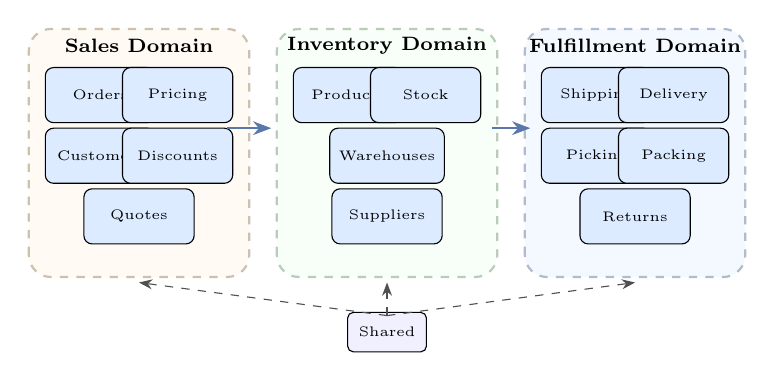
\begin{tikzpicture}[scale=0.7]
        % Domain boundaries
        \draw[thick, dashed, domaincolor!80!black, fill=domaincolor!30, rounded corners=8pt] (-5.5, -1.5) rectangle (-1.5, 3);
        \node[font=\scriptsize\bfseries] at (-3.5, 2.7) {Sales Domain};
        
        \draw[thick, dashed, servicecolor!80!black, fill=servicecolor!30, rounded corners=8pt] (-1, -1.5) rectangle (3, 3);
        \node[font=\scriptsize\bfseries] at (1, 2.7) {Inventory Domain};
        
        \draw[thick, dashed, functionalcolor!80!black, fill=functionalcolor!30, rounded corners=8pt] (3.5, -1.5) rectangle (7.5, 3);
        \node[font=\scriptsize\bfseries] at (5.5, 2.7) {Fulfillment Domain};
        
        % Functional components
        \node[draw, fill=functionalcolor, rounded corners=3pt, minimum width=1.4cm, minimum height=0.7cm, font=\tiny] at (-4.2, 1.8) {Orders};
        \node[draw, fill=functionalcolor, rounded corners=3pt, minimum width=1.4cm, minimum height=0.7cm, font=\tiny] at (-2.8, 1.8) {Pricing};
        \node[draw, fill=functionalcolor, rounded corners=3pt, minimum width=1.4cm, minimum height=0.7cm, font=\tiny] at (-4.2, 0.7) {Customers};
        \node[draw, fill=functionalcolor, rounded corners=3pt, minimum width=1.4cm, minimum height=0.7cm, font=\tiny] at (-2.8, 0.7) {Discounts};
        \node[draw, fill=functionalcolor, rounded corners=3pt, minimum width=1.4cm, minimum height=0.7cm, font=\tiny] at (-3.5, -0.4) {Quotes};
        
        \node[draw, fill=functionalcolor, rounded corners=3pt, minimum width=1.4cm, minimum height=0.7cm, font=\tiny] at (0.3, 1.8) {Products};
        \node[draw, fill=functionalcolor, rounded corners=3pt, minimum width=1.4cm, minimum height=0.7cm, font=\tiny] at (1.7, 1.8) {Stock};
        \node[draw, fill=functionalcolor, rounded corners=3pt, minimum width=1.4cm, minimum height=0.7cm, font=\tiny] at (1, 0.7) {Warehouses};
        \node[draw, fill=functionalcolor, rounded corners=3pt, minimum width=1.4cm, minimum height=0.7cm, font=\tiny] at (1, -0.4) {Suppliers};
        
        \node[draw, fill=functionalcolor, rounded corners=3pt, minimum width=1.4cm, minimum height=0.7cm, font=\tiny] at (4.8, 1.8) {Shipping};
        \node[draw, fill=functionalcolor, rounded corners=3pt, minimum width=1.4cm, minimum height=0.7cm, font=\tiny] at (6.2, 1.8) {Delivery};
        \node[draw, fill=functionalcolor, rounded corners=3pt, minimum width=1.4cm, minimum height=0.7cm, font=\tiny] at (4.8, 0.7) {Picking};
        \node[draw, fill=functionalcolor, rounded corners=3pt, minimum width=1.4cm, minimum height=0.7cm, font=\tiny] at (6.2, 0.7) {Packing};
        \node[draw, fill=functionalcolor, rounded corners=3pt, minimum width=1.4cm, minimum height=0.7cm, font=\tiny] at (5.5, -0.4) {Returns};
        
        % Cross-domain relationships
        \draw[-{Stealth}, thick, secondary] (-1.9, 1.2) -- (-1.1, 1.2);
        \draw[-{Stealth}, thick, secondary] (2.9, 1.2) -- (3.6, 1.2);
        
        % Shared kernel indicator
        \node[draw, fill=datacolor, rounded corners=2pt, minimum width=1cm, minimum height=0.5cm, font=\tiny] at (1, -2.5) {Shared};
        \draw[-{Stealth}, dashed, darkgray] (1, -2.2) -- (-3.5, -1.6);
        \draw[-{Stealth}, dashed, darkgray] (1, -2.2) -- (1, -1.6);
        \draw[-{Stealth}, dashed, darkgray] (1, -2.2) -- (5.5, -1.6);
        
    \end{tikzpicture}
    
    \vspace{1.3cm}
    
    \begin{tabular}{ll}
        \textbf{Version:} & 2.0 \\
        \textbf{Status:} & Release \\
        \textbf{Classification:} & ISO/IEC/IEEE 42010 Compliant \\
        \textbf{Last Updated:} & \today \\
    \end{tabular}
    
    \vfill
    
    {\small Based on the Views and Beyond approach to software architecture documentation}
    
\end{titlepage}

\clearpage
\hypersetup{pageanchor=true}


% -----------------------------------------------------------------------------
% TABLE OF CONTENTS
% -----------------------------------------------------------------------------
\tableofcontents
\newpage

% =============================================================================
% SECTION: VIEWPOINT NAME
% =============================================================================
\section{Viewpoint Name}

\begin{definitionbox}[Viewpoint Identification]
\begin{tabular}{@{}L{3.5cm}L{10cm}@{}}
\textbf{Name:} & Logical Viewpoint \\[0.5em]
\textbf{Synonyms:} & Functional Viewpoint, Domain View, Conceptual Architecture View, Business Capability View, Service View, Functional Decomposition View \\[0.5em]
\textbf{Identifier:} & VP-LOG-001 \\[0.5em]
\textbf{Version:} & 2.0 \\
\end{tabular}
\end{definitionbox}

\subsection{Viewpoint Classification}

The Logical Viewpoint describes the system's functional structure in terms of logical elements, their responsibilities, and relationships---independent of implementation technology. Within the Views and Beyond approach, this aligns with Module styles (particularly Decomposition and Uses) but at a higher abstraction level focusing on functional capabilities rather than code modules. This viewpoint bridges business requirements and technical architecture.

\begin{table}[H]
\centering
\caption{Viewpoint Classification Taxonomy}
\begin{tabular}{@{}L{4cm}L{10cm}@{}}
\toprule
\textbf{Attribute} & \textbf{Value} \\
\midrule
Style Family & Module (Logical/Conceptual) \\
Primary Focus & Functional Elements and Domain Structure \\
Abstraction Level & High-Level / Conceptual \\
Temporal Perspective & Static Functional Structure \\
Related Styles & Decomposition, Layered, Domain-Driven Design \\
IEEE 42010 Category & Functional/Logical Viewpoint \\
4+1 View Model & Logical View \\
\bottomrule
\end{tabular}
\end{table}

\subsection{Viewpoint Scope}

The Logical Viewpoint encompasses the following aspects:

\begin{itemize}
    \item \textbf{Functional Decomposition:} How system functionality is partitioned into logical elements with clear responsibilities.
    
    \item \textbf{Domain Structure:} Organization of the system according to business domains and subdomains.
    
    \item \textbf{Business Capabilities:} Mapping of system elements to business capabilities they enable.
    
    \item \textbf{Logical Services:} Abstract service definitions independent of implementation.
    
    \item \textbf{Information Entities:} Key domain entities and their relationships.
    
    \item \textbf{Functional Dependencies:} How logical elements depend on and interact with each other.
    
    \item \textbf{Domain Boundaries:} Clear boundaries between different functional areas.
    
    \item \textbf{Cross-Cutting Concerns:} Functionality that spans multiple domains.
\end{itemize}

% =============================================================================
% SECTION: OVERVIEW
% =============================================================================
\section{Overview}

The Logical Viewpoint provides a technology-independent view of the system's functional organization. It serves as a bridge between business requirements and technical implementation, ensuring that the system's structure reflects business needs and domain knowledge.

\subsection{Purpose and Scope}

The primary purpose of this viewpoint is to establish a clear functional decomposition that stakeholders from both business and technical backgrounds can understand and validate. It captures the essential "what" of the system before diving into the "how" of implementation.

\begin{definitionbox}[Viewpoint Definition]
The Logical Viewpoint defines the system's functional structure in terms of logical elements, their responsibilities, relationships, and organization into domains. It provides a conceptual model that is independent of specific technologies, platforms, or implementation approaches, focusing on functional capabilities and domain concepts that align with business needs.
\end{definitionbox}

\subsection{Key Characteristics}

The Logical Viewpoint exhibits several distinctive characteristics:

\textbf{Technology Independence:} Describes functionality without reference to specific programming languages, frameworks, or platforms.

\textbf{Business Alignment:} Structure reflects business domains, capabilities, and terminology rather than technical concerns.

\textbf{Stakeholder Accessibility:} Understandable by both business and technical stakeholders, using domain language.

\textbf{Stability:} More stable than implementation views as it changes only when business requirements change.

\textbf{Foundation for Design:} Guides subsequent technical architecture decisions and implementation structure.

\subsection{Relationship to Other Viewpoints}

The Logical Viewpoint connects to other architectural viewpoints:

\begin{table}[H]
\centering
\caption{Relationships to Other Viewpoints}
\begin{tabular}{@{}L{3.5cm}L{10.5cm}@{}}
\toprule
\textbf{Viewpoint} & \textbf{Relationship} \\
\midrule
Context & Context defines external boundaries; Logical defines internal functional structure. \\
\addlinespace
Development & Logical elements guide code module organization. Domain boundaries inform package structure. \\
\addlinespace
Component-and-Connector & Logical services are realized as runtime components. Functional flows become connectors. \\
\addlinespace
Deployment & Logical boundaries may inform deployment unit boundaries. \\
\addlinespace
Information/Data & Domain entities in logical view are detailed in data models. \\
\addlinespace
Process & Functional elements may map to processes or services at runtime. \\
\bottomrule
\end{tabular}
\end{table}

\subsection{Logical Architecture Overview}

\begin{figure}[H]
\centering
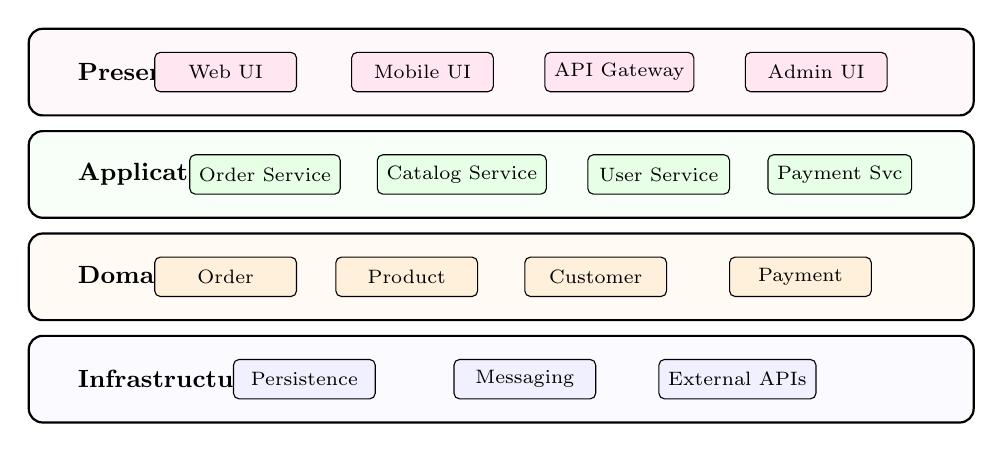
\begin{tikzpicture}[
    node distance=1cm and 1.5cm,
    layer/.style={draw, thick, rounded corners=5pt, minimum width=12cm, minimum height=1.1cm, font=\small},
    element/.style={draw, fill=functionalcolor, rounded corners=2pt, minimum width=1.8cm, minimum height=0.5cm, font=\scriptsize},
]
    % Layers
    \node[layer, fill=interfacecolor!30] (presentation) at (0, 3.5) {};
    \node[font=\small\bfseries, anchor=west] at (-5.5, 3.5) {Presentation};
    
    \node[layer, fill=servicecolor!30] (application) at (0, 2.2) {};
    \node[font=\small\bfseries, anchor=west] at (-5.5, 2.2) {Application Services};
    
    \node[layer, fill=domaincolor!30] (domain) at (0, 0.9) {};
    \node[font=\small\bfseries, anchor=west] at (-5.5, 0.9) {Domain Layer};
    
    \node[layer, fill=datacolor!30] (infrastructure) at (0, -0.4) {};
    \node[font=\small\bfseries, anchor=west] at (-5.5, -0.4) {Infrastructure};
    
    % Presentation elements
    \node[element, fill=interfacecolor] at (-3.5, 3.5) {Web UI};
    \node[element, fill=interfacecolor] at (-1, 3.5) {Mobile UI};
    \node[element, fill=interfacecolor] at (1.5, 3.5) {API Gateway};
    \node[element, fill=interfacecolor] at (4, 3.5) {Admin UI};
    
    % Application elements
    \node[element, fill=servicecolor] at (-3, 2.2) {Order Service};
    \node[element, fill=servicecolor] at (-0.5, 2.2) {Catalog Service};
    \node[element, fill=servicecolor] at (2, 2.2) {User Service};
    \node[element, fill=servicecolor] at (4.3, 2.2) {Payment Svc};
    
    % Domain elements
    \node[element, fill=domaincolor] at (-3.5, 0.9) {Order};
    \node[element, fill=domaincolor] at (-1.2, 0.9) {Product};
    \node[element, fill=domaincolor] at (1.2, 0.9) {Customer};
    \node[element, fill=domaincolor] at (3.8, 0.9) {Payment};
    
    % Infrastructure elements
    \node[element, fill=datacolor] at (-2.5, -0.4) {Persistence};
    \node[element, fill=datacolor] at (0.3, -0.4) {Messaging};
    \node[element, fill=datacolor] at (3, -0.4) {External APIs};
    
\end{tikzpicture}
\caption{Logical Architecture Layers}
\end{figure}

% =============================================================================
% SECTION: CONCERNS
% =============================================================================
\section{Concerns}

This section enumerates the architectural concerns that the Logical Viewpoint is designed to address.

\subsection{Primary Concerns}

\begin{enumerate}[label=\textbf{C\arabic*:}, leftmargin=2.5em]
    \item \textbf{Functional Decomposition}
    \begin{itemize}[nosep]
        \item How is system functionality partitioned?
        \item What are the major functional areas?
        \item What responsibilities does each element have?
        \item How are responsibilities distributed?
        \item What is the rationale for the decomposition?
    \end{itemize}
    
    \item \textbf{Domain Structure}
    \begin{itemize}[nosep]
        \item What business domains does the system address?
        \item How are domains bounded and separated?
        \item What are the core vs supporting domains?
        \item How do domains relate to organizational structure?
        \item What ubiquitous language exists in each domain?
    \end{itemize}
    
    \item \textbf{Business Capability Mapping}
    \begin{itemize}[nosep]
        \item What business capabilities does the system enable?
        \item How do functional elements map to capabilities?
        \item What is the capability maturity in each area?
        \item How do capabilities align with business strategy?
        \item What capability gaps exist?
    \end{itemize}
    
    \item \textbf{Service Identification}
    \begin{itemize}[nosep]
        \item What logical services exist?
        \item What operations does each service provide?
        \item What are service boundaries?
        \item How autonomous are services?
        \item What service contracts exist?
    \end{itemize}
    
    \item \textbf{Domain Entity Modeling}
    \begin{itemize}[nosep]
        \item What are the key domain entities?
        \item What are entity relationships?
        \item What are aggregate boundaries?
        \item What invariants must be maintained?
        \item How do entities map to bounded contexts?
    \end{itemize}
    
    \item \textbf{Functional Dependencies}
    \begin{itemize}[nosep]
        \item How do functional elements depend on each other?
        \item What is the dependency direction?
        \item Are there circular dependencies?
        \item What coupling exists between elements?
        \item How are dependencies managed?
    \end{itemize}
    
    \item \textbf{Information Flow}
    \begin{itemize}[nosep]
        \item How does information flow between elements?
        \item What data is shared vs. private?
        \item What transformations occur?
        \item What is the source of truth for each data type?
        \item How is data consistency maintained?
    \end{itemize}
    
    \item \textbf{Cross-Cutting Functionality}
    \begin{itemize}[nosep]
        \item What functionality spans multiple domains?
        \item How is cross-cutting functionality handled?
        \item What shared services exist?
        \item How are shared concepts managed?
        \item What integration patterns are used?
    \end{itemize}
    
    \item \textbf{Extensibility and Evolution}
    \begin{itemize}[nosep]
        \item How can new functionality be added?
        \item What extension points exist?
        \item How do domains evolve independently?
        \item What backward compatibility is required?
        \item How are breaking changes managed?
    \end{itemize}
    
    \item \textbf{Business Rules and Logic}
    \begin{itemize}[nosep]
        \item Where do business rules reside?
        \item How are rules organized and managed?
        \item What validation logic exists?
        \item How are policies enforced?
        \item How do rules vary by context?
    \end{itemize}
\end{enumerate}

\subsection{Concern-Quality Attribute Mapping}

\begin{table}[H]
\centering
\caption{Concern to Quality Attribute Mapping}
\small
\begin{tabular}{@{}L{3cm}C{1cm}C{1cm}C{1cm}C{1cm}C{1cm}C{1cm}C{1cm}C{1cm}@{}}
\toprule
\textbf{Concern} & \rotatebox{60}{\textbf{Modtic.}} & \rotatebox{60}{\textbf{Maintain.}} & \rotatebox{60}{\textbf{Testtic.}} & \rotatebox{60}{\textbf{Reustic.}} & \rotatebox{60}{\textbf{Underst.}} & \rotatebox{60}{\textbf{Flextic.}} & \rotatebox{60}{\textbf{Interop.}} & \rotatebox{60}{\textbf{Scaltic.}} \\
\midrule
Decomposition & $\bullet$ & $\bullet$ & $\bullet$ & $\circ$ & $\bullet$ & $\circ$ & -- & $\circ$ \\
Domain Structure & $\bullet$ & $\bullet$ & $\circ$ & $\circ$ & $\bullet$ & $\bullet$ & $\circ$ & $\bullet$ \\
Capabilities & $\circ$ & $\circ$ & -- & $\circ$ & $\bullet$ & $\bullet$ & -- & -- \\
Services & $\bullet$ & $\circ$ & $\bullet$ & $\bullet$ & $\circ$ & $\bullet$ & $\bullet$ & $\bullet$ \\
Entities & $\circ$ & $\bullet$ & $\circ$ & $\circ$ & $\bullet$ & $\circ$ & $\circ$ & -- \\
Dependencies & $\bullet$ & $\bullet$ & $\bullet$ & $\circ$ & $\circ$ & $\circ$ & -- & $\circ$ \\
Info Flow & $\circ$ & $\circ$ & $\circ$ & -- & $\circ$ & $\circ$ & $\bullet$ & $\circ$ \\
Cross-Cutting & $\circ$ & $\circ$ & $\circ$ & $\bullet$ & $\circ$ & $\circ$ & $\bullet$ & -- \\
Extenstic. & $\bullet$ & $\circ$ & $\circ$ & $\bullet$ & -- & $\bullet$ & $\circ$ & $\bullet$ \\
Business Rules & $\circ$ & $\bullet$ & $\bullet$ & $\circ$ & $\bullet$ & $\circ$ & -- & -- \\
\bottomrule
\multicolumn{9}{l}{\footnotesize $\bullet$ = Primary impact, $\circ$ = Secondary impact, -- = Minimal impact}
\end{tabular}
\end{table}

% =============================================================================
% SECTION: ANTI-CONCERNS
% =============================================================================
\section{Anti-Concerns}

Understanding what the Logical Viewpoint is \emph{not} appropriate for helps stakeholders avoid misapplying this viewpoint.

\subsection{Out of Scope Topics}

\begin{enumerate}[label=\textbf{AC\arabic*:}, leftmargin=2.5em]
    \item \textbf{Implementation Technology}
    \begin{itemize}[nosep]
        \item Programming languages and frameworks
        \item Database technologies
        \item Messaging platforms
        \item Cloud services
        \item Library choices
    \end{itemize}
    
    \item \textbf{Physical Deployment}
    \begin{itemize}[nosep]
        \item Server configurations
        \item Container orchestration
        \item Network topology
        \item Cloud infrastructure
        \item Environment configurations
    \end{itemize}
    
    \item \textbf{Runtime Behavior}
    \begin{itemize}[nosep]
        \item Process and thread structure
        \item Concurrency mechanisms
        \item Performance optimization
        \item Caching strategies
        \item Resource management
    \end{itemize}
    
    \item \textbf{Detailed Data Models}
    \begin{itemize}[nosep]
        \item Physical database schemas
        \item Index definitions
        \item Storage optimization
        \item Query patterns
        \item Data migration scripts
    \end{itemize}
    
    \item \textbf{Operational Concerns}
    \begin{itemize}[nosep]
        \item Monitoring and alerting
        \item Deployment pipelines
        \item Incident management
        \item Backup and recovery
        \item Security implementation
    \end{itemize}
\end{enumerate}

\begin{warningbox}[Common Misapplications]
Avoid using the Logical Viewpoint for:

\begin{itemize}[nosep]
    \item Specifying implementation details (use Development Viewpoint)
    \item Defining physical deployment (use Deployment Viewpoint)
    \item Detailing runtime components (use C\&C Viewpoint)
    \item Specifying database schemas (use Information Viewpoint)
    \item Documenting API contracts (use Interface Specifications)
\end{itemize}
\end{warningbox}

% =============================================================================
% SECTION: TYPICAL STAKEHOLDERS
% =============================================================================
\section{Typical Stakeholders}

The Logical Viewpoint serves stakeholders across business and technical domains.

\subsection{Primary Stakeholders}

\begin{table}[H]
\centering
\caption{Primary Stakeholder Analysis}
\small
\begin{tabular}{@{}L{2.6cm}L{3.6cm}L{7cm}@{}}
\toprule
\textbf{Stakeholder} & \textbf{Role Description} & \textbf{Primary Interests} \\
\midrule
Software Architects & Design system structure & Functional decomposition, domain boundaries, dependencies \\
\addlinespace
Business Analysts & Define requirements & Business capability mapping, domain terminology \\
\addlinespace
Domain Experts & Provide domain knowledge & Domain model accuracy, business rule placement \\
\addlinespace
Product Managers & Define product direction & Feature placement, capability roadmap \\
\addlinespace
Development Leads & Guide implementation & Service boundaries, module structure guidance \\
\addlinespace
Enterprise Architects & Manage system portfolio & Capability alignment, reuse opportunities \\
\bottomrule
\end{tabular}
\end{table}

\subsection{Secondary Stakeholders}

\begin{table}[H]
\centering
\caption{Secondary Stakeholder Analysis}
\small
\begin{tabular}{@{}L{2.6cm}L{3.6cm}L{7cm}@{}}
\toprule
\textbf{Stakeholder} & \textbf{Role Description} & \textbf{Primary Interests} \\
\midrule
Developers & Implement features & Understanding functional context, responsibility clarity \\
\addlinespace
QA Engineers & Test functionality & Test scope, functional boundaries \\
\addlinespace
Technical Writers & Document system & Domain terminology, functional descriptions \\
\addlinespace
New Team Members & Onboard to system & System understanding, conceptual overview \\
\addlinespace
Integration Teams & Connect systems & Service boundaries, integration points \\
\addlinespace
Business Sponsors & Fund development & Business alignment, capability coverage \\
\bottomrule
\end{tabular}
\end{table}

\subsection{Stakeholder Concern Matrix}

\begin{table}[H]
\centering
\caption{Stakeholder-Concern Responsibility Matrix}
\footnotesize
\begin{tabular}{@{}L{2cm}C{0.8cm}C{0.8cm}C{0.8cm}C{0.8cm}C{0.8cm}C{0.8cm}C{0.8cm}C{0.8cm}C{0.8cm}C{0.8cm}@{}}
\toprule
& \rotatebox{60}{\textbf{Decomp.}} & \rotatebox{60}{\textbf{Domain}} & \rotatebox{60}{\textbf{Capab.}} & \rotatebox{60}{\textbf{Service}} & \rotatebox{60}{\textbf{Entity}} & \rotatebox{60}{\textbf{Depend.}} & \rotatebox{60}{\textbf{InfoFlow}} & \rotatebox{60}{\textbf{CrossCut}} & \rotatebox{60}{\textbf{Extens.}} & \rotatebox{60}{\textbf{Rules}} \\
\midrule
Architect & R & R & C & R & A & R & R & R & R & A \\
Bus. Analyst & C & A & R & C & C & I & C & C & C & R \\
Domain Exp. & C & R & C & I & R & I & C & I & I & R \\
Product Mgr & I & C & A & C & I & I & I & I & A & C \\
Dev Lead & A & C & I & A & C & A & C & A & C & C \\
Enterprise & C & C & R & C & I & C & I & C & C & I \\
\bottomrule
\multicolumn{11}{l}{\footnotesize R = Responsible, A = Accountable, C = Consulted, I = Informed}
\end{tabular}
\end{table}

% =============================================================================
% SECTION: MODEL TYPES
% =============================================================================
\section{Model Types}

The Logical Viewpoint employs several complementary model types to capture different aspects of functional structure.

\subsection{Model Type Catalog}

\begin{enumerate}[label=\textbf{MT\arabic*:}, leftmargin=2.5em]
    \item \textbf{Functional Decomposition Diagram}
    \begin{itemize}[nosep]
        \item \textit{Purpose:} Show hierarchical breakdown of system functionality
        \item \textit{Primary Elements:} Functional areas, sub-functions, relationships
        \item \textit{Key Relationships:} Contains, decomposes-to
        \item \textit{Typical Notation:} Hierarchical diagrams, tree structures
    \end{itemize}
    
    \item \textbf{Domain Model}
    \begin{itemize}[nosep]
        \item \textit{Purpose:} Capture key domain concepts and relationships
        \item \textit{Primary Elements:} Entities, value objects, relationships
        \item \textit{Key Relationships:} Associates, aggregates, inherits
        \item \textit{Typical Notation:} UML class diagrams (conceptual level)
    \end{itemize}
    
    \item \textbf{Bounded Context Map}
    \begin{itemize}[nosep]
        \item \textit{Purpose:} Show domain boundaries and context relationships
        \item \textit{Primary Elements:} Bounded contexts, relationships
        \item \textit{Key Relationships:} Upstream/downstream, shared kernel, ACL
        \item \textit{Typical Notation:} Context map diagrams (DDD style)
    \end{itemize}
    
    \item \textbf{Business Capability Model}
    \begin{itemize}[nosep]
        \item \textit{Purpose:} Map system to business capabilities
        \item \textit{Primary Elements:} Capabilities, capability groups
        \item \textit{Key Relationships:} Enables, supports, requires
        \item \textit{Typical Notation:} Capability maps, heat maps
    \end{itemize}
    
    \item \textbf{Service Catalog}
    \begin{itemize}[nosep]
        \item \textit{Purpose:} Document logical services and operations
        \item \textit{Primary Elements:} Services, operations, contracts
        \item \textit{Key Relationships:} Provides, consumes, depends-on
        \item \textit{Typical Notation:} Service tables, interface diagrams
    \end{itemize}
    
    \item \textbf{Logical Layer Diagram}
    \begin{itemize}[nosep]
        \item \textit{Purpose:} Show functional layers and their relationships
        \item \textit{Primary Elements:} Layers, elements within layers
        \item \textit{Key Relationships:} Uses, calls (top-down only)
        \item \textit{Typical Notation:} Layer diagrams, stack diagrams
    \end{itemize}
    
    \item \textbf{Functional Flow Diagram}
    \begin{itemize}[nosep]
        \item \textit{Purpose:} Show information and control flow between elements
        \item \textit{Primary Elements:} Functions, flows, decision points
        \item \textit{Key Relationships:} Flows-to, triggers, responds-to
        \item \textit{Typical Notation:} Flow diagrams, sequence diagrams
    \end{itemize}
    
    \item \textbf{Use Case Realization}
    \begin{itemize}[nosep]
        \item \textit{Purpose:} Show how functional elements realize use cases
        \item \textit{Primary Elements:} Use cases, participating elements
        \item \textit{Key Relationships:} Participates-in, realizes
        \item \textit{Typical Notation:} Collaboration diagrams, sequence diagrams
    \end{itemize}
    
    \item \textbf{Cross-Reference Matrix}
    \begin{itemize}[nosep]
        \item \textit{Purpose:} Map elements to requirements, capabilities, or domains
        \item \textit{Primary Elements:} Elements, mapping targets
        \item \textit{Key Relationships:} Maps-to, supports, implements
        \item \textit{Typical Notation:} Matrices, tables
    \end{itemize}
\end{enumerate}

\subsection{Model Type Relationships}

\begin{figure}[H]
\centering
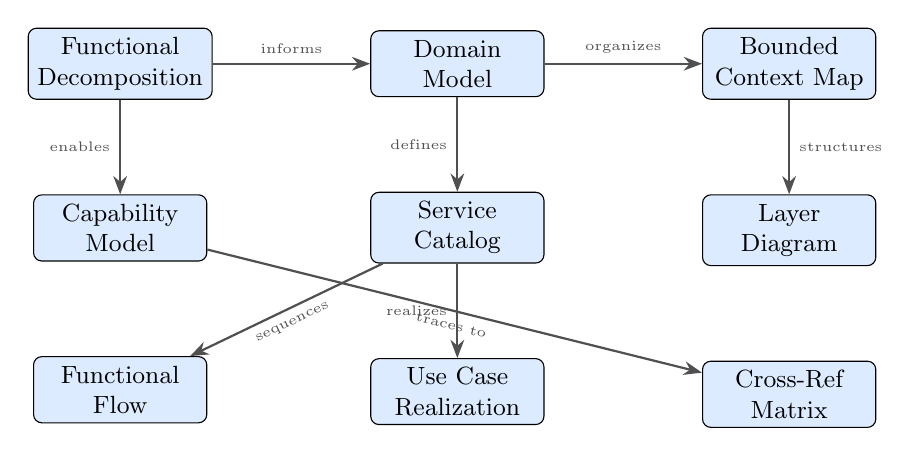
\begin{tikzpicture}[
    node distance=1.2cm and 2cm,
    model/.style={draw, fill=functionalcolor, rounded corners=3pt, minimum width=2.2cm, minimum height=0.7cm, font=\small, align=center},
    arrow/.style={-{Stealth}, thick, darkgray}
]
    % Nodes - top row
    \node[model] (decomp) {Functional\\Decomposition};
    \node[model, right=2cm of decomp] (domain) {Domain\\Model};
    \node[model, right=2cm of domain] (context) {Bounded\\Context Map};
    
    % Nodes - middle row
    \node[model, below=1.2cm of decomp] (capability) {Capability\\Model};
    \node[model, below=1.2cm of domain] (service) {Service\\Catalog};
    \node[model, below=1.2cm of context] (layer) {Layer\\Diagram};
    
    % Nodes - bottom row
    \node[model, below=1.2cm of capability] (flow) {Functional\\Flow};
    \node[model, below=1.2cm of service] (usecase) {Use Case\\Realization};
    \node[model, below=1.2cm of layer] (matrix) {Cross-Ref\\Matrix};
    
    % Arrows
    \draw[arrow] (decomp) -- (domain) node[midway, above, font=\tiny] {informs};
    \draw[arrow] (domain) -- (context) node[midway, above, font=\tiny] {organizes};
    \draw[arrow] (decomp) -- (capability) node[midway, left, font=\tiny] {enables};
    \draw[arrow] (domain) -- (service) node[midway, left, font=\tiny] {defines};
    \draw[arrow] (context) -- (layer) node[midway, right, font=\tiny] {structures};
    \draw[arrow] (service) -- (flow) node[midway, below, sloped, font=\tiny] {sequences};
    \draw[arrow] (service) -- (usecase) node[midway, left, font=\tiny] {realizes};
    \draw[arrow] (capability) -- (matrix) node[midway, below, sloped, font=\tiny] {traces to};
\end{tikzpicture}
\caption{Model Type Dependency Relationships}
\end{figure}

% =============================================================================
% SECTION: MODEL LANGUAGES
% =============================================================================
\section{Model Languages}

For each model type, specific languages, notations, and techniques are prescribed.

\subsection{Logical Element Notation}

\begin{figure}[H]
\centering
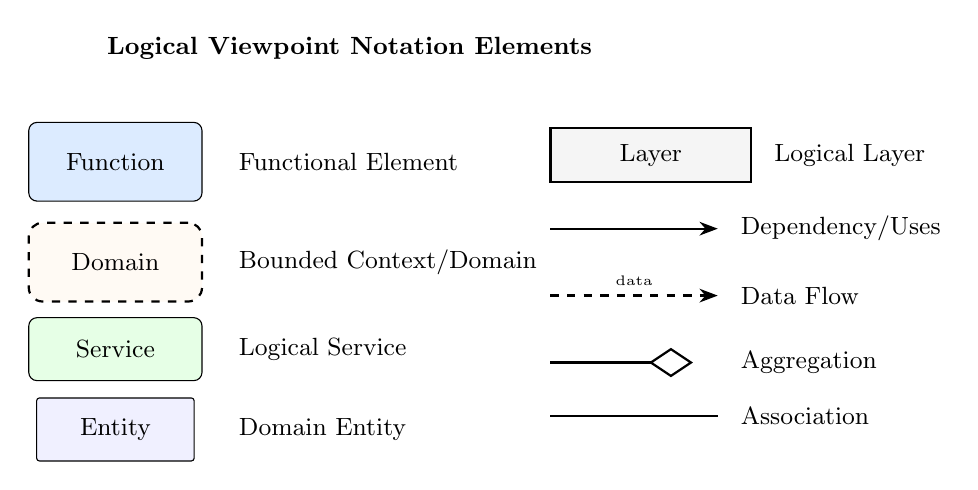
\begin{tikzpicture}[scale=0.85]
    % Legend title
    \node[font=\small\bfseries] at (0, 5) {Logical Viewpoint Notation Elements};
    
    % Functional element
    \node[draw, fill=functionalcolor, rounded corners=3pt, minimum width=2.2cm, minimum height=1cm] at (-3.5, 3.3) {};
    \node[font=\small] at (-3.5, 3.3) {Function};
    \node[right, font=\small] at (-1.8, 3.3) {Functional Element};
    
    % Domain
    \node[draw, thick, dashed, fill=domaincolor!30, rounded corners=5pt, minimum width=2.2cm, minimum height=1cm] at (-3.5, 1.8) {};
    \node[font=\small] at (-3.5, 1.8) {Domain};
    \node[right, font=\small] at (-1.8, 1.8) {Bounded Context/Domain};
    
    % Service
    \node[draw, fill=servicecolor, rounded corners=3pt, minimum width=2.2cm, minimum height=0.8cm] at (-3.5, 0.5) {};
    \node[font=\small] at (-3.5, 0.5) {Service};
    \node[right, font=\small] at (-1.8, 0.5) {Logical Service};
    
    % Entity
    \node[draw, fill=datacolor, rounded corners=1pt, minimum width=2cm, minimum height=0.8cm] at (-3.5, -0.7) {};
    \node[font=\small] at (-3.5, -0.7) {Entity};
    \node[right, font=\small] at (-1.8, -0.7) {Domain Entity};
    
    % Layer
    \draw[thick, fill=layercolor] (3, 3.8) rectangle (6, 3);
    \node[font=\small] at (4.5, 3.4) {Layer};
    \node[right, font=\small] at (6.2, 3.4) {Logical Layer};
    
    % Dependency
    \draw[-{Stealth}, thick] (3, 2.3) -- (5.5, 2.3);
    \node[right, font=\small] at (5.7, 2.3) {Dependency/Uses};
    
    % Flow
    \draw[-{Stealth}, thick, dashed] (3, 1.3) -- (5.5, 1.3);
    \node[above, font=\tiny] at (4.25, 1.3) {data};
    \node[right, font=\small] at (5.7, 1.3) {Data Flow};
    
    % Aggregation
    \draw[thick] (3, 0.3) -- (4.5, 0.3);
    \draw[thick, fill=white] (4.5, 0.3) -- (4.8, 0.5) -- (5.1, 0.3) -- (4.8, 0.1) -- cycle;
    \node[right, font=\small] at (5.7, 0.3) {Aggregation};
    
    % Association
    \draw[thick] (3, -0.5) -- (5.5, -0.5);
    \node[right, font=\small] at (5.7, -0.5) {Association};
    
\end{tikzpicture}
\caption{Logical Viewpoint Notation Legend}
\end{figure}

\subsection{Domain-Driven Design Context Relationships}

\begin{table}[H]
\centering
\caption{DDD Context Relationship Types}
\small
\begin{tabular}{@{}L{2.8cm}L{4.5cm}L{5.5cm}@{}}
\toprule
\textbf{Relationship} & \textbf{Description} & \textbf{When to Use} \\
\midrule
Shared Kernel & Shared subset of domain model & Teams collaborate closely, shared concepts \\
\addlinespace
Customer-Supplier & Upstream serves downstream & Clear dependency direction \\
\addlinespace
Conformist & Downstream conforms to upstream & No control over upstream model \\
\addlinespace
Anti-Corruption Layer & Translation layer between contexts & Protect domain from external model \\
\addlinespace
Open Host Service & Published well-defined protocol & Multiple consumers need access \\
\addlinespace
Published Language & Common interchange format & Cross-system communication \\
\addlinespace
Separate Ways & No integration & Independent development \\
\addlinespace
Partnership & Coordinated evolution & Mutual dependency, joint success \\
\bottomrule
\end{tabular}
\end{table}

\subsection{Functional Element Classification}

\begin{table}[H]
\centering
\caption{Functional Element Type Classification}
\small
\begin{tabular}{@{}L{2.5cm}L{4cm}L{6.5cm}@{}}
\toprule
\textbf{Element Type} & \textbf{Description} & \textbf{Examples} \\
\midrule
Core Domain & Central business differentiator & Order Management, Pricing Engine \\
\addlinespace
Supporting & Supports core without differentiating & Reporting, Notifications \\
\addlinespace
Generic & Commodity, not business-specific & Authentication, File Storage \\
\addlinespace
Application Service & Orchestrates domain operations & OrderProcessingService \\
\addlinespace
Domain Service & Domain logic not in entities & PricingCalculator \\
\addlinespace
Infrastructure & Technical capabilities & EmailSender, DataAccess \\
\bottomrule
\end{tabular}
\end{table}

\subsection{Tabular Specifications}

\subsubsection{Service Specification Table}

\begin{table}[H]
\centering
\caption{Example Service Specification Format}
\small
\begin{tabular}{@{}L{2.2cm}L{2.5cm}L{4cm}L{3.8cm}@{}}
\toprule
\textbf{Service} & \textbf{Domain} & \textbf{Responsibilities} & \textbf{Key Operations} \\
\midrule
Order Service & Sales & Order lifecycle management & createOrder, cancelOrder, getOrder \\
\addlinespace
Pricing Service & Sales & Calculate prices and discounts & calculatePrice, applyDiscount \\
\addlinespace
Inventory Svc & Inventory & Stock management & checkStock, reserveStock, release \\
\addlinespace
Fulfillment Svc & Fulfillment & Order fulfillment coordination & pickOrder, packOrder, shipOrder \\
\bottomrule
\end{tabular}
\end{table}

\subsubsection{Domain Entity Specification Table}

\begin{table}[H]
\centering
\caption{Example Domain Entity Specification}
\small
\begin{tabular}{@{}L{2cm}L{2cm}L{3cm}L{3cm}L{2.5cm}@{}}
\toprule
\textbf{Entity} & \textbf{Domain} & \textbf{Key Attributes} & \textbf{Invariants} & \textbf{Aggregate} \\
\midrule
Order & Sales & id, customer, items, status & Items $>$ 0, valid status & Order (root) \\
\addlinespace
OrderItem & Sales & product, quantity, price & Quantity $>$ 0 & Order \\
\addlinespace
Customer & Sales & id, name, email, tier & Valid email format & Customer (root) \\
\addlinespace
Product & Inventory & sku, name, price, stock & Price $>$ 0 & Product (root) \\
\bottomrule
\end{tabular}
\end{table}

\subsubsection{Capability Mapping Table}

\begin{table}[H]
\centering
\caption{Example Business Capability Mapping}
\small
\begin{tabular}{@{}L{3cm}L{3cm}L{3cm}L{3.5cm}@{}}
\toprule
\textbf{Capability} & \textbf{Sub-Capability} & \textbf{Functional Element} & \textbf{Maturity} \\
\midrule
Sales Management & Order Processing & Order Service & High \\
 & Pricing & Pricing Service & Medium \\
 & Quotations & Quote Service & Low \\
\addlinespace
Inventory Mgmt & Stock Control & Inventory Service & High \\
 & Replenishment & Supplier Service & Medium \\
\addlinespace
Fulfillment & Shipping & Shipping Service & High \\
 & Returns & Returns Service & Medium \\
\bottomrule
\end{tabular}
\end{table}

% =============================================================================
% SECTION: VIEWPOINT METAMODELS
% =============================================================================
\section{Viewpoint Metamodels}

This section defines the conceptual metamodel underlying the Logical Viewpoint.

\subsection{Core Metamodel}

\begin{figure}[H]
\centering
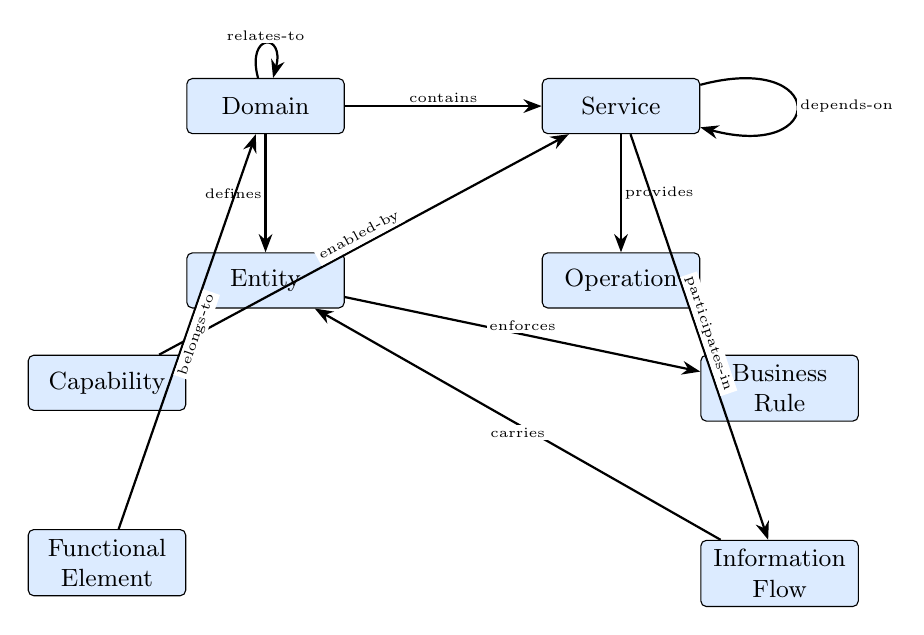
\begin{tikzpicture}[
    node distance=1.3cm and 2cm,
    entity/.style={draw, fill=functionalcolor, rounded corners=2pt, minimum width=2cm, minimum height=0.7cm, font=\small, align=center},
    arrow/.style={-{Stealth}, thick},
    label/.style={font=\tiny, fill=white, inner sep=1pt}
]
    % Main entities
    \node[entity] (domain) {Domain};
    \node[entity, right=2.5cm of domain] (service) {Service};
    \node[entity, below=1.5cm of domain] (entity) {Entity};
    \node[entity, below=1.5cm of service] (operation) {Operation};
    \node[entity, below left=2.8cm and 0cm of domain] (capability) {Capability};
    \node[entity, below right=2.8cm and 0cm of service] (rule) {Business\\Rule};
    \node[entity, below=1.5cm of capability] (function) {Functional\\Element};
    \node[entity, below=1.5cm of rule] (flow) {Information\\Flow};
    
    % Relationships
    \draw[arrow] (domain) -- (service) node[label, midway, above] {contains};
    \draw[arrow] (domain) -- (entity) node[label, midway, left] {defines};
    \draw[arrow] (service) -- (operation) node[label, midway, right] {provides};
    \draw[arrow] (entity) -- (rule) node[label, midway, above] {enforces};
    \draw[arrow] (capability) -- (service) node[label, midway, above, sloped] {enabled-by};
    \draw[arrow] (function) -- (domain) node[label, midway, below, sloped] {belongs-to};
    \draw[arrow] (service) -- (flow) node[label, midway, above, sloped] {participates-in};
    \draw[arrow] (flow) -- (entity) node[label, midway, below] {carries};
    
    % Self-reference
    \draw[arrow] (domain) to[loop above] node[label, above] {relates-to} (domain);
    \draw[arrow] (service) to[loop right] node[label, right] {depends-on} (service);
\end{tikzpicture}
\caption{Logical Viewpoint Core Metamodel}
\end{figure}

\subsection{Entity Definitions}

\begin{definitionbox}[Entity: Domain]
\textbf{Definition:} A bounded context representing a cohesive area of business functionality with its own ubiquitous language, model, and boundaries.

\textbf{Attributes:}
\begin{itemize}[nosep]
    \item \texttt{domainId}: Unique identifier
    \item \texttt{name}: Domain name
    \item \texttt{description}: Domain purpose and scope
    \item \texttt{type}: Domain type (core, supporting, generic)
    \item \texttt{ubiquitousLanguage}: Key terms and definitions
    \item \texttt{owner}: Team or individual responsible
    \item \texttt{boundaries}: What is in/out of scope
    \item \texttt{subdomains}: Child domains if decomposed
    \item \texttt{contextRelationships}: Relationships to other domains
\end{itemize}

\textbf{Constraints:}
\begin{itemize}[nosep]
    \item Domain must have clear boundaries
    \item Ubiquitous language must be documented
    \item Core domains must be identified and prioritized
    \item Context relationships must be explicitly defined
\end{itemize}
\end{definitionbox}

\begin{definitionbox}[Entity: Service]
\textbf{Definition:} A logical grouping of related operations that provides a cohesive set of capabilities, encapsulating domain logic behind a well-defined interface.

\textbf{Attributes:}
\begin{itemize}[nosep]
    \item \texttt{serviceId}: Unique identifier
    \item \texttt{name}: Service name
    \item \texttt{description}: Service purpose
    \item \texttt{domain}: Owning domain
    \item \texttt{type}: Service type (application, domain, infrastructure)
    \item \texttt{operations}: List of operations provided
    \item \texttt{dependencies}: Services this depends on
    \item \texttt{consumers}: Services that consume this
    \item \texttt{contracts}: Interface contracts
    \item \texttt{autonomy}: Level of independence
\end{itemize}

\textbf{Constraints:}
\begin{itemize}[nosep]
    \item Service must belong to exactly one domain
    \item Operations must be cohesive to service purpose
    \item Dependencies should follow domain relationships
    \item Contracts must be versioned
\end{itemize}
\end{definitionbox}

\begin{definitionbox}[Entity: Domain Entity]
\textbf{Definition:} A domain object with identity that encapsulates state and behavior, representing a key concept within a bounded context.

\textbf{Attributes:}
\begin{itemize}[nosep]
    \item \texttt{entityId}: Unique identifier
    \item \texttt{name}: Entity name
    \item \texttt{description}: Entity purpose
    \item \texttt{domain}: Owning domain
    \item \texttt{attributes}: Key attributes
    \item \texttt{relationships}: Relationships to other entities
    \item \texttt{invariants}: Business rules that must hold
    \item \texttt{lifecycle}: Valid lifecycle states
    \item \texttt{aggregate}: Aggregate this belongs to (if any)
    \item \texttt{isAggregateRoot}: Whether this is an aggregate root
\end{itemize}

\textbf{Constraints:}
\begin{itemize}[nosep]
    \item Entity must have identity
    \item Invariants must be enforceable
    \item Aggregate boundaries must be clear
    \item Lifecycle states must be well-defined
\end{itemize}
\end{definitionbox}

\begin{definitionbox}[Entity: Operation]
\textbf{Definition:} A specific action or behavior that a service can perform, representing a unit of functionality with defined inputs and outputs.

\textbf{Attributes:}
\begin{itemize}[nosep]
    \item \texttt{operationId}: Unique identifier
    \item \texttt{name}: Operation name (verb-noun format)
    \item \texttt{description}: Operation purpose
    \item \texttt{service}: Owning service
    \item \texttt{inputs}: Input parameters
    \item \texttt{outputs}: Output/return values
    \item \texttt{preconditions}: Required state before execution
    \item \texttt{postconditions}: Guaranteed state after execution
    \item \texttt{exceptions}: Possible failure conditions
    \item \texttt{idempotent}: Whether operation is idempotent
\end{itemize}

\textbf{Constraints:}
\begin{itemize}[nosep]
    \item Operation name should clearly indicate action
    \item Inputs and outputs must be documented
    \item Side effects should be explicit
\end{itemize}
\end{definitionbox}

\begin{definitionbox}[Entity: Capability]
\textbf{Definition:} A business ability that the system enables, representing what the business can do (not how it does it).

\textbf{Attributes:}
\begin{itemize}[nosep]
    \item \texttt{capabilityId}: Unique identifier
    \item \texttt{name}: Capability name
    \item \texttt{description}: Capability purpose
    \item \texttt{level}: Hierarchy level (L1, L2, L3)
    \item \texttt{parent}: Parent capability (if any)
    \item \texttt{children}: Child capabilities
    \item \texttt{enablingServices}: Services that enable this
    \item \texttt{maturity}: Current maturity level
    \item \texttt{strategicImportance}: Business importance
    \item \texttt{owner}: Business owner
\end{itemize}

\textbf{Constraints:}
\begin{itemize}[nosep]
    \item Capabilities should be business-focused, not technical
    \item Hierarchy should be consistent
    \item Strategic capabilities should be identified
\end{itemize}
\end{definitionbox}

\begin{definitionbox}[Entity: Business Rule]
\textbf{Definition:} A constraint, policy, or logic that governs business operations and must be enforced by the system.

\textbf{Attributes:}
\begin{itemize}[nosep]
    \item \texttt{ruleId}: Unique identifier
    \item \texttt{name}: Rule name
    \item \texttt{description}: Rule statement
    \item \texttt{type}: Rule type (constraint, derivation, policy)
    \item \texttt{domain}: Domain where rule applies
    \item \texttt{entities}: Entities affected by rule
    \item \texttt{expression}: Formal rule expression
    \item \texttt{enforcement}: Where/how rule is enforced
    \item \texttt{source}: Business source of rule
    \item \texttt{exceptions}: Allowed exceptions
\end{itemize}

\textbf{Constraints:}
\begin{itemize}[nosep]
    \item Rules must be clearly stated
    \item Enforcement location must be defined
    \item Business source should be traceable
\end{itemize}
\end{definitionbox}

\begin{definitionbox}[Entity: Functional Element]
\textbf{Definition:} A logical unit of functionality that contributes to system capabilities, abstracting implementation details.

\textbf{Attributes:}
\begin{itemize}[nosep]
    \item \texttt{elementId}: Unique identifier
    \item \texttt{name}: Element name
    \item \texttt{description}: Element purpose
    \item \texttt{domain}: Owning domain
    \item \texttt{type}: Element type (core, supporting, infrastructure)
    \item \texttt{responsibilities}: Key responsibilities
    \item \texttt{dependencies}: Elements this depends on
    \item \texttt{interfaces}: Provided/required interfaces
    \item \texttt{constraints}: Applicable constraints
\end{itemize}

\textbf{Constraints:}
\begin{itemize}[nosep]
    \item Element should have single clear responsibility
    \item Dependencies should be minimized
    \item Interfaces should be well-defined
\end{itemize}
\end{definitionbox}

\begin{definitionbox}[Entity: Information Flow]
\textbf{Definition:} The movement of data or messages between functional elements, characterizing how information is exchanged.

\textbf{Attributes:}
\begin{itemize}[nosep]
    \item \texttt{flowId}: Unique identifier
    \item \texttt{name}: Flow name
    \item \texttt{description}: Flow purpose
    \item \texttt{source}: Origin element
    \item \texttt{destination}: Target element
    \item \texttt{dataType}: Type of information carried
    \item \texttt{trigger}: What initiates the flow
    \item \texttt{frequency}: How often flow occurs
    \item \texttt{synchronicity}: Sync vs async
    \item \texttt{transformation}: Any data transformation
\end{itemize}

\textbf{Constraints:}
\begin{itemize}[nosep]
    \item Flows should have clear purpose
    \item Data types should be well-defined
    \item Cross-domain flows should be explicit
\end{itemize}
\end{definitionbox}

\subsection{Relationship Definitions}

\begin{table}[H]
\centering
\caption{Metamodel Relationship Definitions}
\small
\begin{tabular}{@{}L{2.3cm}L{1.8cm}L{1.8cm}L{7.5cm}@{}}
\toprule
\textbf{Relationship} & \textbf{Source} & \textbf{Target} & \textbf{Description} \\
\midrule
contains & Domain & Service & Domain includes this service \\
\addlinespace
defines & Domain & Entity & Domain defines this entity \\
\addlinespace
provides & Service & Operation & Service offers this operation \\
\addlinespace
enforces & Entity & Rule & Entity enforces this business rule \\
\addlinespace
enabled-by & Capability & Service & Capability is enabled by service \\
\addlinespace
belongs-to & Function & Domain & Functional element is in domain \\
\addlinespace
depends-on & Service & Service & Service requires another service \\
\addlinespace
participates-in & Service & Flow & Service is part of information flow \\
\addlinespace
carries & Flow & Entity & Flow transmits entity data \\
\addlinespace
relates-to & Domain & Domain & Domain has relationship to another \\
\bottomrule
\end{tabular}
\end{table}

% =============================================================================
% SECTION: CONFORMING NOTATIONS
% =============================================================================
\section{Conforming Notations}

Several existing notations and modeling approaches align with the Logical Viewpoint.

\subsection{UML Structural Diagrams}

UML provides several diagram types suitable for logical modeling:

\textbf{Class Diagrams (Conceptual):} Domain entities, relationships, and attributes at a conceptual level.

\textbf{Package Diagrams:} Grouping of elements into domains and functional areas.

\textbf{Component Diagrams:} Logical components and their dependencies (abstract level).

\textbf{Conformance Level:} High for domain modeling, medium for service modeling.

\subsection{Domain-Driven Design Notations}

DDD provides specialized notations for bounded contexts and strategic design:

\textbf{Context Maps:} Show relationships between bounded contexts.

\textbf{Aggregate Diagrams:} Show aggregate boundaries and roots.

\textbf{Conformance Level:} High for domain structure and boundaries.

\subsection{ArchiMate}

ArchiMate provides enterprise architecture notation including business and application layers:

\textbf{Business Layer:} Capabilities, processes, functions.

\textbf{Application Layer:} Application services, components, interfaces.

\textbf{Conformance Level:} High for capability modeling and layered views.

\subsection{Notation Comparison}

\begin{table}[H]
\centering
\caption{Logical Notation Comparison}
\small
\begin{tabular}{@{}L{2.5cm}C{1.2cm}C{1.2cm}C{1.2cm}C{1.2cm}C{1.2cm}C{1.2cm}@{}}
\toprule
\textbf{Feature} & \rotatebox{60}{\textbf{UML}} & \rotatebox{60}{\textbf{DDD}} & \rotatebox{60}{\textbf{ArchiMate}} & \rotatebox{60}{\textbf{BPMN}} & \rotatebox{60}{\textbf{SysML}} & \rotatebox{60}{\textbf{Custom}} \\
\midrule
Domain modeling & $\bullet$ & $\bullet$ & $\circ$ & -- & $\circ$ & $\bullet$ \\
Service definition & $\circ$ & $\circ$ & $\bullet$ & $\circ$ & $\circ$ & $\bullet$ \\
Capability mapping & -- & -- & $\bullet$ & -- & $\circ$ & $\bullet$ \\
Context boundaries & $\circ$ & $\bullet$ & $\bullet$ & -- & $\circ$ & $\bullet$ \\
Entity modeling & $\bullet$ & $\bullet$ & $\circ$ & -- & $\bullet$ & $\bullet$ \\
Flow modeling & $\circ$ & -- & $\circ$ & $\bullet$ & $\bullet$ & $\bullet$ \\
Layering & $\circ$ & $\circ$ & $\bullet$ & -- & $\circ$ & $\bullet$ \\
Standardized & $\bullet$ & $\circ$ & $\bullet$ & $\bullet$ & $\bullet$ & -- \\
\bottomrule
\multicolumn{7}{l}{\footnotesize $\bullet$ = Strong support, $\circ$ = Limited support, -- = Not applicable}
\end{tabular}
\end{table}

% =============================================================================
% SECTION: MODEL CORRESPONDENCE RULES
% =============================================================================
\section{Model Correspondence Rules}

Model correspondence rules define how elements in logical models relate to elements in other architectural views.

\subsection{Development View Correspondence}

\begin{definitionbox}[Correspondence Rule CR-01: Domain to Package Mapping]
\textbf{Rule:} Every domain should map to one or more code packages/modules in the development view.

\textbf{Formal Expression:}
\begin{center}
$\forall d \in Domains : \exists P \subseteq Packages : implements(P, d)$
\end{center}

\textbf{Rationale:} Ensures domain boundaries are reflected in code structure.

\textbf{Verification:} Package structure review.
\end{definitionbox}

\begin{definitionbox}[Correspondence Rule CR-02: Service to Module Mapping]
\textbf{Rule:} Every logical service must be implemented by code modules.

\textbf{Formal Expression:}
\begin{center}
$\forall s \in Services : \exists M \subseteq Modules : realizes(M, s)$
\end{center}

\textbf{Rationale:} Ensures services have implementation.

\textbf{Verification:} Traceability matrix.
\end{definitionbox}

\subsection{Component-and-Connector View Correspondence}

\begin{definitionbox}[Correspondence Rule CR-03: Service to Component Mapping]
\textbf{Rule:} Logical services should map to runtime components.

\textbf{Formal Expression:}
\begin{center}
$\forall s \in Services : \exists c \in Components : manifests(c, s)$
\end{center}

\textbf{Rationale:} Ensures logical design is realized at runtime.

\textbf{Verification:} Component traceability review.
\end{definitionbox}

\subsection{Information View Correspondence}

\begin{definitionbox}[Correspondence Rule CR-04: Entity to Data Model Mapping]
\textbf{Rule:} Domain entities should have corresponding elements in data models.

\textbf{Formal Expression:}
\begin{center}
$\forall e \in DomainEntities : \exists d \in DataEntities : represents(d, e)$
\end{center}

\textbf{Rationale:} Ensures domain concepts are persisted.

\textbf{Verification:} Data model review.
\end{definitionbox}

% =============================================================================
% SECTION: OPERATIONS ON VIEWS
% =============================================================================
\section{Operations on Views}

This section defines methods for creating, interpreting, analyzing, and maintaining logical views.

\subsection{Creation Methods}

\subsubsection{View Development Process}

\begin{guidancebox}[Step 1: Identify Business Domains]
\begin{enumerate}[nosep]
    \item Analyze business processes and organizational structure
    \item Identify major functional areas
    \item Determine core vs supporting vs generic domains
    \item Define domain boundaries
    \item Document ubiquitous language for each domain
\end{enumerate}
\end{guidancebox}

\begin{guidancebox}[Step 2: Model Domain Entities]
\begin{enumerate}[nosep]
    \item Identify key domain concepts in each domain
    \item Define entity attributes and relationships
    \item Identify aggregate boundaries
    \item Document entity invariants
    \item Define entity lifecycles
\end{enumerate}
\end{guidancebox}

\begin{guidancebox}[Step 3: Define Services]
\begin{enumerate}[nosep]
    \item Group related operations into services
    \item Define service responsibilities
    \item Identify service dependencies
    \item Document service contracts
    \item Assess service autonomy
\end{enumerate}
\end{guidancebox}

\begin{guidancebox}[Step 4: Map Business Capabilities]
\begin{enumerate}[nosep]
    \item Define capability hierarchy
    \item Map services to capabilities
    \item Assess capability maturity
    \item Identify capability gaps
    \item Prioritize capability development
\end{enumerate}
\end{guidancebox}

\begin{guidancebox}[Step 5: Define Context Relationships]
\begin{enumerate}[nosep]
    \item Identify domain interactions
    \item Choose appropriate relationship types
    \item Define integration patterns
    \item Document shared concepts
    \item Plan translation layers
\end{enumerate}
\end{guidancebox}

\begin{guidancebox}[Step 6: Document Business Rules]
\begin{enumerate}[nosep]
    \item Gather rules from domain experts
    \item Classify rules by type
    \item Assign rules to domains/entities
    \item Define enforcement mechanisms
    \item Document exceptions
\end{enumerate}
\end{guidancebox}

\begin{guidancebox}[Step 7: Validate and Refine]
\begin{enumerate}[nosep]
    \item Review with domain experts
    \item Validate against requirements
    \item Check for completeness
    \item Assess coupling and cohesion
    \item Refine based on feedback
\end{enumerate}
\end{guidancebox}

\subsubsection{Domain Decomposition Strategies}

\begin{patternbox}[Strategy: Business Capability Decomposition]
\textbf{Approach:} Structure domains around business capabilities.

\textbf{Process:}
\begin{enumerate}[nosep]
    \item Define L1 business capabilities
    \item Decompose into L2, L3 capabilities
    \item Group capabilities into domains
    \item Align domains with capability ownership
\end{enumerate}

\textbf{Use When:} Strong alignment with business organization needed.
\end{patternbox}

\begin{patternbox}[Strategy: Event Storming]
\textbf{Approach:} Discover domains through domain events.

\textbf{Process:}
\begin{enumerate}[nosep]
    \item Identify domain events (orange stickies)
    \item Group events by aggregate (yellow)
    \item Identify bounded contexts from clusters
    \item Define context relationships
\end{enumerate}

\textbf{Use When:} Collaborative discovery with domain experts.
\end{patternbox}

\begin{patternbox}[Strategy: Value Stream Decomposition]
\textbf{Approach:} Align domains with value streams.

\textbf{Process:}
\begin{enumerate}[nosep]
    \item Map end-to-end value streams
    \item Identify value-adding activities
    \item Group activities into domains
    \item Optimize for flow
\end{enumerate}

\textbf{Use When:} Focus on customer value delivery.
\end{patternbox}

\subsection{Analysis Methods}

\subsubsection{Coupling and Cohesion Analysis}

\begin{definitionbox}[Cohesion Assessment]
\textbf{Purpose:} Evaluate how well elements within a domain belong together.

\textbf{High Cohesion Indicators:}
\begin{itemize}[nosep]
    \item Elements share common purpose
    \item Elements change together
    \item Elements use shared terminology
    \item Elements owned by same team
\end{itemize}

\textbf{Low Cohesion Indicators:}
\begin{itemize}[nosep]
    \item Mixed responsibilities
    \item Unrelated elements grouped together
    \item Different change drivers
    \item Terminology confusion
\end{itemize}
\end{definitionbox}

\begin{definitionbox}[Coupling Assessment]
\textbf{Purpose:} Evaluate dependencies between domains/services.

\textbf{Coupling Types (least to most problematic):}
\begin{enumerate}[nosep]
    \item \textbf{Message coupling:} Communication via messages
    \item \textbf{Data coupling:} Sharing data structures
    \item \textbf{Control coupling:} Sharing control logic
    \item \textbf{Content coupling:} Direct internal access
\end{enumerate}

\textbf{Reduction Strategies:}
\begin{itemize}[nosep]
    \item Use anti-corruption layers
    \item Define explicit contracts
    \item Prefer asynchronous communication
    \item Duplicate data to reduce runtime coupling
\end{itemize}
\end{definitionbox}

% =============================================================================
% SECTION: EXAMPLES
% =============================================================================
\section{Examples}

\subsection{Example 1: E-Commerce Domain Model}

\begin{figure}[H]
\centering
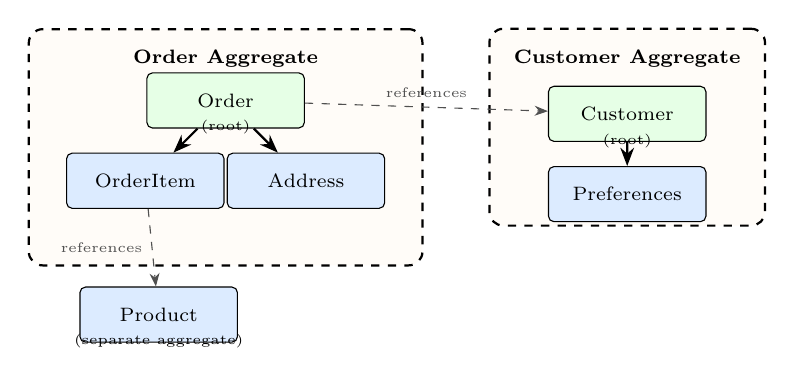
\begin{tikzpicture}[
    entity/.style={draw, fill=functionalcolor, rounded corners=2pt, minimum width=2cm, minimum height=0.7cm, font=\scriptsize},
    aggregate/.style={draw, thick, dashed, rounded corners=5pt, fill=domaincolor!20},
    scale=0.85
]
    % Order Aggregate
    \node[aggregate, minimum width=5cm, minimum height=3cm] (orderagg) at (-3, 0) {};
    \node[font=\scriptsize\bfseries, anchor=north] at (-3, 1.6) {Order Aggregate};
    
    \node[entity, fill=servicecolor] (order) at (-3, 0.7) {Order};
    \node[font=\tiny] at (-3, 0.3) {(root)};
    \node[entity] (item) at (-4.2, -0.5) {OrderItem};
    \node[entity] (addr) at (-1.8, -0.5) {Address};
    
    % Customer Aggregate
    \node[aggregate, minimum width=3.5cm, minimum height=2.5cm] (custagg) at (3, 0.3) {};
    \node[font=\scriptsize\bfseries, anchor=north] at (3, 1.6) {Customer Aggregate};
    
    \node[entity, fill=servicecolor] (cust) at (3, 0.5) {Customer};
    \node[font=\tiny] at (3, 0.1) {(root)};
    \node[entity] (pref) at (3, -0.7) {Preferences};
    
    % Relationships
    \draw[-{Stealth}, thick] (order) -- (item);
    \draw[-{Stealth}, thick] (order) -- (addr);
    \draw[-{Stealth}, thick] (cust) -- (pref);
    \draw[-{Stealth}, dashed, darkgray] (order) -- (cust) node[midway, above, font=\tiny] {references};
    
    % Product (separate)
    \node[entity] (prod) at (-4, -2.5) {Product};
    \node[font=\tiny] at (-4, -2.9) {(separate aggregate)};
    \draw[-{Stealth}, dashed, darkgray] (item) -- (prod) node[midway, left, font=\tiny] {references};
    
\end{tikzpicture}
\caption{E-Commerce Domain Model with Aggregates}
\end{figure}

\textbf{Description:} This domain model shows two aggregates: Order and Customer. Order is the aggregate root containing OrderItem and Address. Customer is a separate aggregate referenced by Order (not contained). Product is in a separate aggregate and only referenced by OrderItem via ID.

\subsection{Example 2: Bounded Context Map}

\begin{figure}[H]
\centering
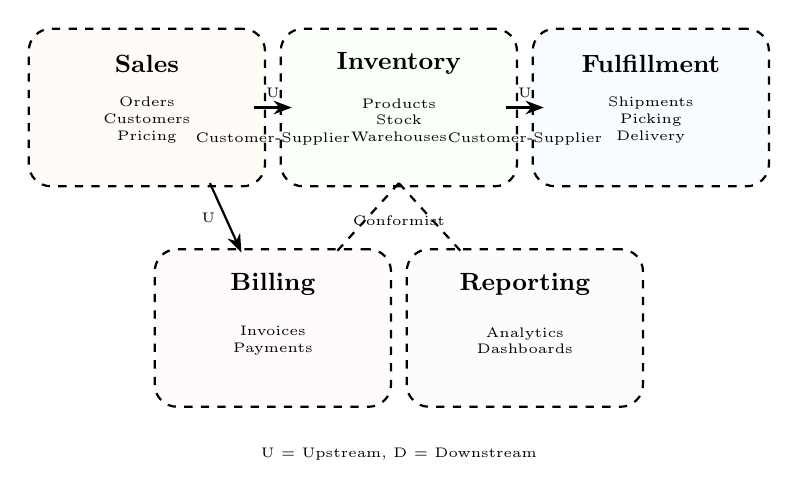
\begin{tikzpicture}[
    context/.style={draw, thick, dashed, rounded corners=8pt, minimum width=3cm, minimum height=2cm, fill=#1!20},
    scale=0.8
]
    % Contexts
    \node[context=domaincolor] (sales) at (-4, 2) {};
    \node[font=\small\bfseries] at (-4, 2.7) {Sales};
    \node[font=\tiny, align=center] at (-4, 1.8) {Orders\\Customers\\Pricing};
    
    \node[context=servicecolor] (inventory) at (0, 2) {};
    \node[font=\small\bfseries] at (0, 2.7) {Inventory};
    \node[font=\tiny, align=center] at (0, 1.8) {Products\\Stock\\Warehouses};
    
    \node[context=functionalcolor] (fulfillment) at (4, 2) {};
    \node[font=\small\bfseries] at (4, 2.7) {Fulfillment};
    \node[font=\tiny, align=center] at (4, 1.8) {Shipments\\Picking\\Delivery};
    
    \node[context=interfacecolor] (billing) at (-2, -1.5) {};
    \node[font=\small\bfseries] at (-2, -0.8) {Billing};
    \node[font=\tiny, align=center] at (-2, -1.7) {Invoices\\Payments};
    
    \node[context=datacolor] (reporting) at (2, -1.5) {};
    \node[font=\small\bfseries] at (2, -0.8) {Reporting};
    \node[font=\tiny, align=center] at (2, -1.7) {Analytics\\Dashboards};
    
    % Relationships
    \draw[-{Stealth}, thick] (-2.3, 2) -- (-1.7, 2) node[midway, above, font=\tiny] {U};
    \node[font=\tiny] at (-2, 1.5) {Customer-Supplier};
    
    \draw[-{Stealth}, thick] (1.7, 2) -- (2.3, 2) node[midway, above, font=\tiny] {U};
    \node[font=\tiny] at (2, 1.5) {Customer-Supplier};
    
    \draw[-{Stealth}, thick] (-3, 0.8) -- (-2.5, -0.3) node[midway, left, font=\tiny] {U};
    
    \draw[thick, dashed] (0, 0.8) -- (-1, -0.3);
    \draw[thick, dashed] (0, 0.8) -- (1, -0.3);
    \node[font=\tiny] at (0, 0.2) {Conformist};
    
    % Legend
    \node[font=\tiny] at (0, -3.5) {U = Upstream, D = Downstream};
    
\end{tikzpicture}
\caption{Bounded Context Map}
\end{figure}

\textbf{Description:} This context map shows five bounded contexts with their relationships. Sales is upstream to Inventory and Billing. Inventory is upstream to Fulfillment. Reporting is a conformist to both Sales and Inventory, meaning it conforms to their models without translation.

\subsection{Example 3: Business Capability Heat Map}

\begin{table}[H]
\centering
\caption{Business Capability Maturity Heat Map}
\small
\begin{tabular}{@{}L{3cm}L{3cm}C{2cm}C{2cm}C{2cm}@{}}
\toprule
\textbf{L1 Capability} & \textbf{L2 Capability} & \textbf{Maturity} & \textbf{Strategic} & \textbf{Investment} \\
\midrule
\multirow{3}{*}{Customer Mgmt} & Acquisition & \cellcolor{green!30}High & Yes & Maintain \\
 & Retention & \cellcolor{yellow!30}Medium & Yes & Grow \\
 & Support & \cellcolor{green!30}High & No & Maintain \\
\midrule
\multirow{3}{*}{Order Mgmt} & Order Entry & \cellcolor{green!30}High & Yes & Maintain \\
 & Order Tracking & \cellcolor{yellow!30}Medium & No & Grow \\
 & Returns & \cellcolor{red!30}Low & No & Build \\
\midrule
\multirow{3}{*}{Inventory Mgmt} & Stock Control & \cellcolor{green!30}High & No & Maintain \\
 & Forecasting & \cellcolor{red!30}Low & Yes & Build \\
 & Replenishment & \cellcolor{yellow!30}Medium & No & Grow \\
\bottomrule
\end{tabular}
\end{table}

% =============================================================================
% SECTION: NOTES
% =============================================================================
\section{Notes}

\subsection{Domain-Driven Design Principles}

\begin{domainbox}[Strategic DDD Guidelines]
\begin{itemize}[nosep]
    \item \textbf{Focus on Core Domain:} Invest most effort in differentiating capabilities
    \item \textbf{Ubiquitous Language:} Use consistent terminology from domain experts
    \item \textbf{Bounded Contexts:} Clearly define model boundaries
    \item \textbf{Context Mapping:} Explicitly define how contexts relate
    \item \textbf{Anti-Corruption Layers:} Protect domain model from external influences
    \item \textbf{Shared Kernel:} Carefully manage shared code between contexts
    \item \textbf{Continuous Refinement:} Evolve model as understanding deepens
\end{itemize}
\end{domainbox}

\subsection{Service Design Principles}

\begin{functionalbox}[Service Design Guidelines]
\begin{itemize}[nosep]
    \item \textbf{Single Responsibility:} Each service has one clear purpose
    \item \textbf{Loose Coupling:} Minimize dependencies between services
    \item \textbf{High Cohesion:} Related operations belong together
    \item \textbf{Explicit Contracts:} Clear interface definitions
    \item \textbf{Encapsulation:} Hide internal implementation
    \item \textbf{Autonomy:} Services can operate independently
    \item \textbf{Statelessness:} Prefer stateless service design where possible
\end{itemize}
\end{functionalbox}

\subsection{Common Pitfalls}

\begin{warningbox}[Common Mistakes to Avoid]
\begin{enumerate}[nosep]
    \item \textbf{Anemic Domain Model:} Entities with only data, no behavior
    \item \textbf{God Services:} Services doing too much
    \item \textbf{Leaky Abstractions:} Implementation details in logical models
    \item \textbf{Ignoring Bounded Contexts:} Trying to create single unified model
    \item \textbf{Technology-Driven Design:} Letting tools drive domain structure
    \item \textbf{Missing Ubiquitous Language:} Inconsistent terminology
    \item \textbf{Premature Decomposition:} Splitting before understanding
    \item \textbf{Circular Dependencies:} Creating dependency cycles between domains
\end{enumerate}
\end{warningbox}

% =============================================================================
% SECTION: SOURCES
% =============================================================================
\section{Sources}

\subsection{Primary References}

\begin{enumerate}
    \item Clements, P., et al. (2010). \textit{Documenting Software Architectures: Views and Beyond} (2nd ed.). Addison-Wesley Professional.
    
    \item Evans, E. (2003). \textit{Domain-Driven Design: Tackling Complexity in the Heart of Software}. Addison-Wesley Professional.
    
    \item Vernon, V. (2013). \textit{Implementing Domain-Driven Design}. Addison-Wesley Professional.
    
    \item Rozanski, N., \& Woods, E. (2011). \textit{Software Systems Architecture} (2nd ed.). Addison-Wesley Professional.
    
    \item Bass, L., Clements, P., \& Kazman, R. (2021). \textit{Software Architecture in Practice} (4th ed.). Addison-Wesley Professional.
\end{enumerate}

\subsection{Supplementary References}

\begin{enumerate}[resume]
    \item Vernon, V. (2016). \textit{Domain-Driven Design Distilled}. Addison-Wesley Professional.
    
    \item Brandolini, A. (2021). \textit{Introducing EventStorming}. Leanpub.
    
    \item Newman, S. (2021). \textit{Building Microservices} (2nd ed.). O'Reilly Media.
    
    \item Fowler, M. (2002). \textit{Patterns of Enterprise Application Architecture}. Addison-Wesley Professional.
    
    \item The Open Group. (2018). \textit{ArchiMate 3.1 Specification}.
\end{enumerate}

\subsection{Online Resources}

\begin{itemize}
    \item Domain-Driven Design Reference: \url{https://www.domainlanguage.com/ddd/reference/}
    \item Martin Fowler's Patterns: \url{https://martinfowler.com/}
    \item EventStorming: \url{https://www.eventstorming.com/}
    \item Microservices.io Patterns: \url{https://microservices.io/patterns/}
    \item ArchiMate: \url{https://www.opengroup.org/archimate-forum}
\end{itemize}

% =============================================================================
% APPENDIX
% =============================================================================
\appendix

\section{Logical View Checklist}

\begin{table}[H]
\centering
\small
\begin{tabular}{@{}L{10cm}C{2cm}@{}}
\toprule
\textbf{Item} & \textbf{Complete?} \\
\midrule
\multicolumn{2}{l}{\textbf{Domain Structure}} \\
\quad Business domains identified & $\square$ \\
\quad Domain boundaries defined & $\square$ \\
\quad Core/supporting/generic classification done & $\square$ \\
\quad Ubiquitous language documented & $\square$ \\
\quad Context relationships mapped & $\square$ \\
\midrule
\multicolumn{2}{l}{\textbf{Domain Entities}} \\
\quad Key entities identified & $\square$ \\
\quad Entity relationships defined & $\square$ \\
\quad Aggregate boundaries established & $\square$ \\
\quad Entity invariants documented & $\square$ \\
\quad Lifecycles defined & $\square$ \\
\midrule
\multicolumn{2}{l}{\textbf{Services}} \\
\quad Services identified and documented & $\square$ \\
\quad Service responsibilities defined & $\square$ \\
\quad Service dependencies mapped & $\square$ \\
\quad Contracts documented & $\square$ \\
\midrule
\multicolumn{2}{l}{\textbf{Business Alignment}} \\
\quad Capabilities mapped & $\square$ \\
\quad Business rules documented & $\square$ \\
\quad Requirements traced & $\square$ \\
\quad Domain expert review completed & $\square$ \\
\midrule
\multicolumn{2}{l}{\textbf{Quality}} \\
\quad Cohesion assessed & $\square$ \\
\quad Coupling minimized & $\square$ \\
\quad Dependencies are acyclic & $\square$ \\
\quad Extension points identified & $\square$ \\
\bottomrule
\end{tabular}
\end{table}

\section{Glossary}

\begin{description}[style=nextline, leftmargin=3cm, labelwidth=2.8cm]
    \item[Aggregate] A cluster of domain objects treated as a unit for data changes.
    
    \item[Aggregate Root] The entity that serves as the entry point to an aggregate.
    
    \item[Bounded Context] A boundary within which a domain model is defined and applicable.
    
    \item[Business Capability] An ability that a business possesses or needs.
    
    \item[Cohesion] The degree to which elements of a module belong together.
    
    \item[Context Map] A diagram showing relationships between bounded contexts.
    
    \item[Coupling] The degree of interdependence between modules.
    
    \item[Domain] A sphere of knowledge or activity.
    
    \item[Domain Entity] An object defined by its identity rather than attributes.
    
    \item[Domain Service] A service that encapsulates domain logic not belonging to entities.
    
    \item[Functional Element] A logical unit of system functionality.
    
    \item[Invariant] A condition that must always be true for an object.
    
    \item[Service] A logical grouping of operations providing business capabilities.
    
    \item[Ubiquitous Language] A common language shared by developers and domain experts.
    
    \item[Value Object] An object defined by its attributes, with no identity.
\end{description}

% =============================================================================
% END DOCUMENT
% =============================================================================

\end{document}
